\documentclass[signature=data]{physicsreport}

%%
%% User settings
%%

\classno{}
\stuno{}
\groupno{}
\stuname{}
\expdate{\expdatefmt\today}
\expname{用示波器观测磁滞回线}

%%
%% Document body
%%

\begin{document}
% First page
% Some titles and personal information are defined in ``\maketitle''.
\maketitle

\section{实验目的}
\section{实验预习}


% Teacher signature
\makeatletter
\physicsreport@body@signature{preparation}
\makeatother


% Original experiment data
\section{实验现象及原始数据记录}


% Teacher signature
\makeatletter
\physicsreport@body@signature{data}
\makeatother

\newpage
% Data process and others
\section{数据处理及作图}

根据$U_x$与$H$之间的关系和$U_y$与$B$之间的关系及相关数据,可以计算得到数据并绘制各样品的磁滞回线。用python画图如下:

\begin{figure}[H]
    \centering
    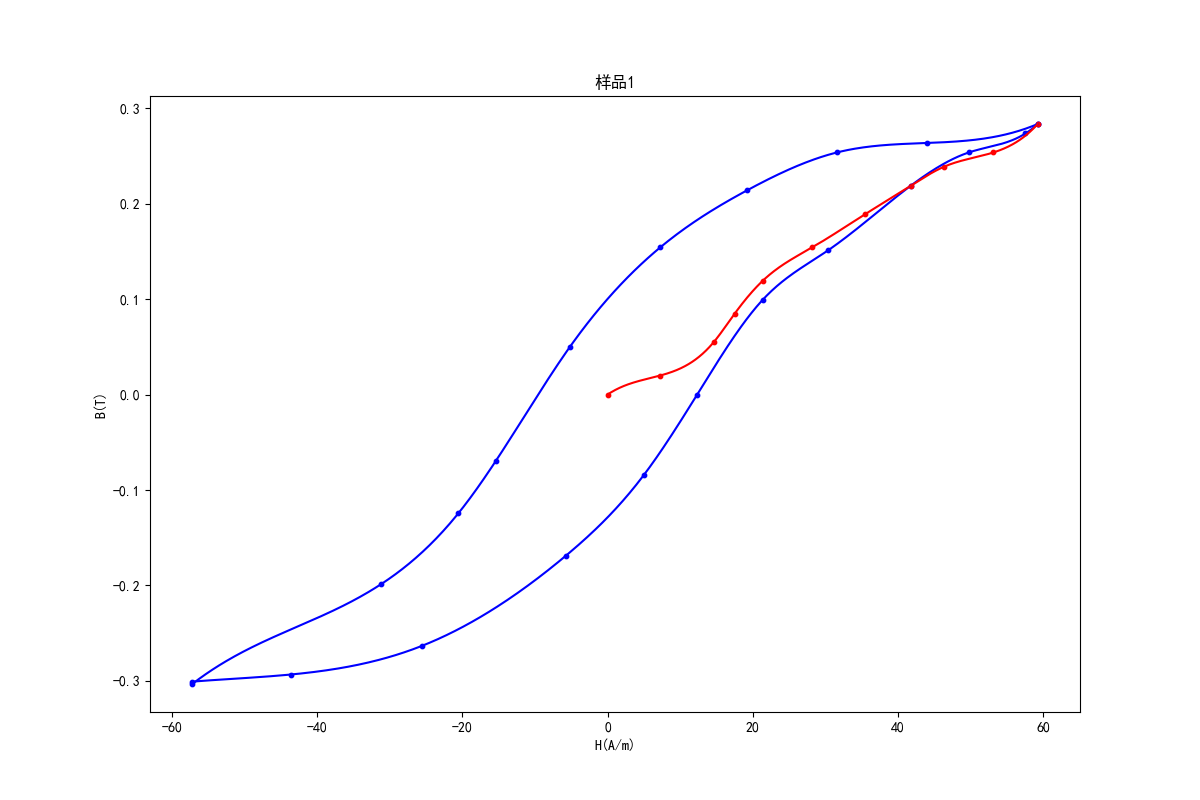
\includegraphics[width=0.8\textwidth]{images/lab15/Figure_1.png}
\end{figure}

\begin{figure}[H]
    \centering
    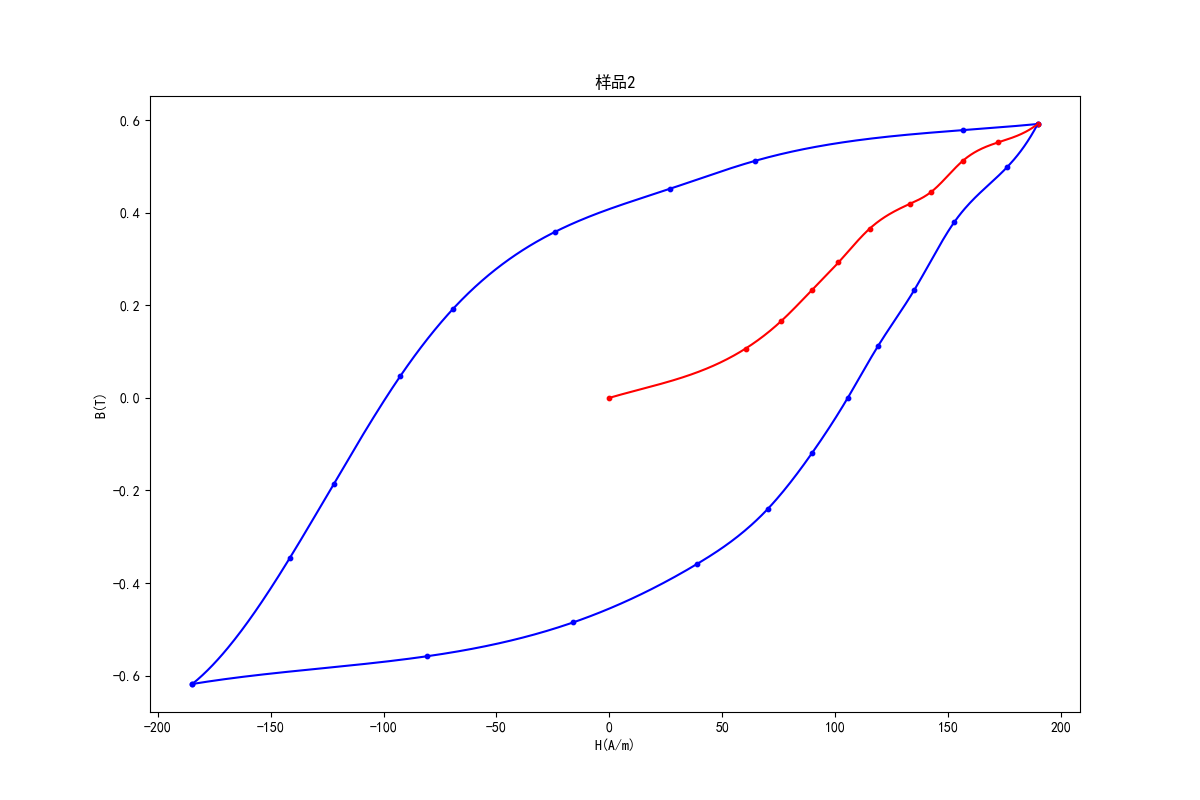
\includegraphics[width=0.8\textwidth]{images/lab15/Figure_2.png}
\end{figure}

\newpage

\section{实验结论及现象分析}

由实验测量数据和公式$U_x=\frac{LR_1}{N_1}H$与$U_y=\frac{N_2S}{R_2C}B$可以计算得到,

样品 1 的剩磁为 $0.126 T$,矫顽⼒为 $16.1 A/m$;

样品 2 的剩磁为 $0.401 T$,矫顽⼒为 $101.4 A/m$。

数据与图对照,发现在误差允许的范围内,实验数据与理论值符合较好。



\section{讨论问题}




\end{document}